\newcommand{\CLASSINPUTinnersidemargin}{18mm}
\newcommand{\CLASSINPUToutersidemargin}{12mm}
\newcommand{\CLASSINPUTtoptextmargin}{20mm}
\newcommand{\CLASSINPUTbottomtextmargin}{25mm}
\documentclass[10pt,conference,a4paper]{IEEEtran}
%%%%%%%%%%%%%%%%%%%%%%%%%%%%%%%%%%%%%%%%%%%%%%%%%%%%%%%%%%%%%%%%%%%%%%%%%%%%%%%%

% Para que salgan las cosas en castellano (tildes, notaci�n decimal...)
\usepackage[latin1]{inputenc}
\usepackage[english]{babel}
% \usepackage[utf8x]{inputenc} 

% % Intenta corregir los efectos indeseados de babel
% \renewcommand{\thesubsection}{\Alph{subsection}}
% \renewcommand{\thesubsubsection}{\arabic{subsubsection}}
% \addto\extrasspanish{\def\tablename{Tabla}}
% \addto\extrasspanish{\def\figurename{Fig.}}

% Fuente Times...
\usepackage{times}

\usepackage{graphicx}
% % figuras en formato .png, .ps, pdf � eps
% \DeclareGraphicsExtensions{.png,.eps,.ps,.pdf}

%Otros paquetes que pueden resultar de inter�s
\usepackage{amsmath}
\usepackage{amsfonts}
\usepackage{amssymb}
\usepackage{cite}

% algorithm typesetting
\usepackage{algorithm}
\usepackage{algpseudocode}

% control the spacing before and after the equations
\setlength{\abovedisplayskip}{0pt} \setlength{\belowdisplayskip}{0pt}
\setlength{\abovedisplayshortskip}{0pt} \setlength{\belowdisplayshortskip}{0pt}

\newcommand{\B}{\mathcal{B}}
\newcommand{\Bin}{\mathcal{B}_{\text{in}}}
\newcommand{\Bout}{\mathcal{B}_{\text{out}}}

\newcommand{\tx}{\text{tx}}
\newcommand{\C}{\mathbb{C}}
\newcommand{\R}{\mathbb{R}}

\newcommand{\x}{\mathbf{x}}
\newcommand{\y}{\mathbf{y}}
\newcommand{\n}{\mathbf{n}}
% \H is already defined, so use \HH to represent the channel matrix
\newcommand{\HH}{\mathbf{H}}
\newcommand{\QQ}{\mathbf{Q}}
\newcommand{\0}{\mathbf{0}}
\newcommand{\1}{\mathbf{1}}
\newcommand{\I}{\mathbf{I}}
\newcommand{\W}{\mathbf{W}}
\newcommand{\w}{\mathbf{w}}
% \P is already defined, so use \PP to represent the power assignment matrix
\newcommand{\PP}{\mathbf{P}}
\newcommand{\s}{\mathbf{s}}

\newcommand{\U}{\mathbf{U}}
\newcommand{\D}{\mathbf{S}}
\newcommand{\V}{\mathbf{V}}

\newcommand{\A}{\mathbf{A}}

\newcommand{\refs}[1]{Section~\ref{#1}}
\newcommand{\reff}[1]{Figure~\ref{#1}}
\newcommand{\refa}[1]{Algorithm~\ref{#1}}

\DeclareMathOperator*{\argmax}{arg\,max}
\DeclareMathOperator*{\first}{first}
\DeclareMathOperator*{\cell}{cell}

\begin{document}

\title{Adaptive Block Diagonalization and User Scheduling With Out of Cluster Interference}

% Nombres y direcciones de los autores

\author{
\authorblockN{Juan Jos� Garc�a Fern�ndez$^\ast$, Ana Garc�a Armada$^\ast$, Javier Rubio$^\dagger$}
\authorblockN{Antonio Pascual-Iserte$^\dagger$, Oriol Font-Bach$^\ddagger$, Nikolaos Bartzoudis$^\ddagger$}
\authorblockA{$^\ast$Dept. Signal Theory and Communications, Universidad Carlos III de Madrid (UC3M), Madrid, Spain.}
\authorblockA{$^\dagger$Dept. Signal Theory and Communications, Universitat Polit�cnica de Catalunya (UPC), Barcelona, Spain.}
\authorblockA{$^\ddagger$Centre Tecnol�gic de Telecomunicacions de Catalunya (CTTC), Castelldefels, Spain.}
\authorblockA{Emails: \{jjgarcia, agarcia\}@tsc.uc3m.es, \{javier.rubio.lopez, antonio.pascual\}@upc.edu, \{ofont, nbartzoudis\}@cttc.cat}
}

\maketitle

{\let\thefootnote\relax\footnotetext{The research leading to these results has received funding from the Spanish Ministry of Economy and Competitiveness (Ministerio de Econom�a y Competitividad) under projects TEC2011-29006-C03-01 (GRE3N-PHY), TEC2011-29006-C03-02 (GRE3N-LINK-MAC), TEC2011-29006-C03-03 (GRE3N-SYST).}}

\begin{abstract}
	Interference in a cellular network is one of the main impairments that needs to be overcome. Coordination among the Base Stations may enable the use of the interference to improve the transmission rate at the cost of increased computational complexity and more stringent backhaul and feedback requirements. Practical problems of global coordination can be reduced through clustering which, in turn, will introduce \emph{Out of Cluster Interference} (OCI). OCI can seriously hamper the advantages brought by precoding techniques like \emph{Block Diagonalization} (BD). In this work we propose a mixed transmission strategy using BD and Single User transmission that is able to overcome the problems introduced by the OCI, in combination with a low complexity scheduling algorithm that enables an increased transmission rate in a multiuser scenario.
\end{abstract}

%%%%%%%%
\section{Introduction}\label{sec:introduction}
Traditionally, cellular networks have dealt with interference in the simplest way possible: trying to avoid it. The latest cellular technologies, like LTE-Advanced, with its enormous peak data requirements, make it necessary to use all resources as efficiently as possible. A ``new look at interference'' \cite{gesbert10} is needed, in the sense that interference should start being used to improve the communications instead of trying to fight it.

Current cellular technologies like LTE define an interface (X2) interconnecting the BS. This interface may enable \emph{Base Stations} (BS) coordination, which can achieve huge gains in terms of data rate \cite{foschini06}. In this direction, Dirty Paper Coding has been shown to provide the maximum capacity for the Gaussian Broadcast Channel \cite{caire03}, but its complexity prevents it from being used in real scenarios. Simpler linear techniques, such as \emph{Block Diagonalization} \cite{spencer04} (BD) can provide important gains with a much lower complexity, making it a more attractive candidate for practical implementations.

Nevertheless, when the size of the cellular network grows, global coordination becomes impractical, due to the increased feedback and backhaul requirements. Additionally, there exist theoretical works that show how the gains from coordination are intrinsically limited for an increasing network size \cite{lozano13}.

Clustering, \cite{papadogiannis10} \cite{baracca12} \cite{mingyi13} \cite{lakshmana12} \cite{gong11}, appears then as a viable option to cope with these limitations. By organizing the network in small groups or clusters, within which the coordination is performed, the complexity and natural limitations of cooperation are reduced. The main drawback of clustering is the presence of \emph{Out of Cluster Interference} (OCI), which is not always considered in the literature. In \cite{zhang09} and \cite{shim08} the OCI is analyzed in the context of a clustered network using BD, and theoretical and asymptotic results are given, albeit without immediate practical applications. In particular, it is shown how BD performs poorly in presence of the OCI. Recent works on clustering and resource allocation as \cite{hosseini13} deal with the OCI through distributed power control. They assume, though, a very common simplification which is a sum power constraint for all the BS in the clusters, something not likely to be achievable in reality.

The problem considered in this paper is the performance loss of BD when OCI is present. A simple and practical algorithm is presented, based on a hybrid strategy combining BD and \emph{Single User} (SU) processing. The best transmisssion scheme is chosen according to a metric that is compared to a simple threshold at each user equipment. The scenario considered is a multi-user one, with each cell serving multiple users. A low complexity algorithm is proposed to schedule the users, trying to take advantage of the multiuser diversity to increase the mean rate per user. In \cite{shen06} a similar suboptimal algorithm, based on the Frobenius norm of the channel matrix is proposed, but it is not analyzed in the presence of OCI, nor it is combined with a hybrid precoding strategy.

The rest of the paper is organized as follows: \refs{sec:system_model} introduces the system model used, followed by \refs{sec:transmission_strategy} where the mix of transmission strategies is described. The scheduling algorithm is presented in \refs{sec:scheduling}, the results of the simulations analyzed in \refs{sec:performance}, and conclusions are drawn in \refs{sec:conclusions}.

%%%%%%%%
\section{System Model}\label{sec:system_model}
This work focuses on the downlink of a cellular network with a set $\B = \Bin \cup \Bout$ of cells. $\Bin$ contains the $M$ cells that form a cluster, and $\Bout$ represents the cells external to the cluster. The $M$ cells from the cluster serve $N$ users. Each BS has $t$ transmitting antennas, while each of the users has $r$ receiving antennas. 

It will be considered that each user is associated to one BS, so that the signal received at the $i$-th user is given by 

\begin{equation}\label{eq:received_signal}
	\y_i = \HH_{ii} \x_i + \underbrace{\sum\limits_{j \in \Bin \backslash \{i\}} \HH_{ij} \x_j}_{\text{Inner interference}} + \underbrace{\sum\limits_{k \in \Bout} \HH_{ik} \x_k}_{\text{OCI}} + \n_i
\end{equation}

\noindent
where $\HH_{im} \in \C^{r\times t}$ is the channel matrix between the $m$-th transmitter and the $i$-th user, $\x_m \in \C^{t\times 1}$ is the signal transmitted at the $m$-th BS, and $\n_i \in \C^{r\times 1}$ is the \emph{additive white gaussian noise} (AWGN) with zero mean and variance $\sigma_i$, $\n_i \sim \mathcal{N}\left(0, \sigma_i\I\right)$ at the $i$-th receiver. Throughout the paper, without loss of generality, it will be assumed that the noise variance is the same for all the users, $\sigma_i = \sigma$.

The rate obtained at the $i$-th receiver is the given by

\begin{equation}\label{eq:rate_original}
	\begin{aligned}
	R_i = \log_2 \left\vert\vphantom{\sum\limits_{j}} \right. & \I + \HH_{ii}\QQ_{i}\HH_{ii}^H \\
	&\left.\left(\sum\limits_{j \in \B \backslash \{i\}}\HH_{ij}\QQ_j\HH_{ij}^H + \sigma^2\I\right)^{-1}\right\vert
	\end{aligned}
\end{equation}

\noindent
where $\QQ_i = \text{E}\left\{\x_i\x_i^H\right\}$ is the covariance matrix of the signal transmitted by the the $i$-th BS.

If no coordination is used, and provided that perfect \emph{channel state information} (CSI) is available at the transmitter, the \emph{singular value decomposition} (SVD) of the channel matrix can be used at each BS to maximize the rate of the user it is serving \cite{telatar99}:

\begin{align*}
	\HH_{ii} &= \U_i \mathbf{\Lambda}_i \V_i^H \\
		\W_i & = \V_i \\
	 \x_i &= \W_i \s_i
\end{align*}

\noindent
where $\W_i \in \C^{t\times r}$ is the precoding matrix used at the $i$-th transmitter, and $\s_i \in \C^{r\times 1}$ is the data intended for user $i$. If at the $i$-th receiver $\U_i^H$ is used as the receiving filter, then the achievable rate becomes

\begin{equation}\label{eq:rate_su}
	\begin{aligned}
	&R_i^{(SU)} = \\
	&\log_2 \left\vert\I + \mathbf{\Lambda}_i \PP_i \left(\sum\limits_{j \in \B \backslash \{i\}}\HH_{ij}\QQ_j\HH_{ij}^H + \sigma^2\I\right)^{-1}\right\vert
	\end{aligned}
\end{equation}

\noindent
where $\PP_i = \text{E}\left\{\s_i\s_i^H\right\} = \text{diag}\left\{p_{i1}, \ldots, p_{ir}\right\}$, is the power assigned to each of the data streams of the $i$-th user.

For the coordination of the $M$ BS in $\Bin$ coordinate to transmit jointly to the $M$ (out of the total $N$) users, it will be used BD \cite{spencer04}, and therefore the rate can be expressed as

\begin{equation}\label{eq:rate_bd}
	\begin{aligned}
	&R_i^{(BD)} = \\
	&\log_2 \left\vert\I + \widetilde{\mathbf{\Lambda}}_i \widetilde{\PP}_i \left(\sum\limits_{j \in \Bout}\HH_{ij}\QQ_j\HH_{ij}^H + \sigma^2\I\right)^{-1}\right\vert
	\end{aligned}
\end{equation}

\noindent
where $\widetilde{\mathbf{\Lambda}}_i$ is the diagonal matrix resulting from applying BD to the cluster channel matrix.

%%%%%%%%
\section{Transmission strategy}\label{sec:transmission_strategy}

OCI can deteriorate the performance of BD, so it is important to find a way of measuring the OCI and mitigating its effects.

In \cite{moon13} they propose a method based on a result in \cite{zhang10} that states that the maximum capacity of a MISO downlink channel can be reached using a combination of two transmission techniques. They are able to find a closed form expression for a threshold for the \emph{signal to interference plus noise ratio} (SINR). This threshold allows each user to individually and locally decide the most convenient transmission strategy.
\cite{zuleita09} presents a similar result to that of \cite{zhang10} for the MIMO case, but the solution is somewhat complicated and it does not allow for the closed form expression for the threshold. In the current work, a similar approach to that in \cite{moon13} will be used, with a metric that will be compared with a fixed threshold locally at each user.

Intuitively, BD will perform better when the OCI is low compared to the power received from the BSs in the cluster. Hence, the metric that will be considered is:

\begin{equation}\label{eq:metric}
\gamma_i = \frac{\sum\limits_{j \in \Bin}\text{Tr}\left(\HH_{ij}\widehat{\PP}_{j}\HH_{ij}^H\right)}{\sum\limits_{j \in \Bout}\text{Tr}\left(\HH_{ij}\widehat{\PP}_{j}\HH_{ij}^H\right)}
\end{equation}

\noindent
where $\text{Tr}(\cdot)$ is the trace of a matrix, and $\widehat{\PP}_{j}$ is a diagonal matrix with the power transmitted through all the antennas of each transmitter.

This metric is compared with a fixed threshold $\gamma_{th}$ for which there is no closed form expression. That is the reason why the threshold considered in this work is calculated through simulations and it is assumed to be known by all the users, the details of how the threshold is calculated are given in \refs{sec:performance}. Each user computes the metric \eqref{eq:metric}, locally, and compares it with the threshold so that if $\gamma_i > \gamma_{th}$ the user chooses BD as transmission strategy, and if $\gamma_i \leq \gamma_{th}$ it opts to choose SU. This information is then sent back to the BS, and it is used by the BSs in the cluster to coordinate the scheduling of the users and the transmission strategy used for each of them.

%%%%%%%%
\section{Scheduling}\label{sec:scheduling}

After the users have made their decision and fed it back to the BS, these will know which users are more suitable to being served using BD and which ones using SU.

The approach followed will be similar to that in \cite{moon13}, where users are grouped so that the transmission strategy in all the BS is the same within a given transmission interval. In \cite{moon13}, this strategy was proposed for simplicity. Here, it is proposed to guarantee a good performance, in the sense that users served with SU may not be affected by other cells in the cluster using BD, but users being served using BD will experience a much more degraded performance if not all the BS in the cluster coordinate, i.e. some of the BS transmit to their users using SU precoding.

As mentioned before, users that are better to be served using SU are indifferent to other users' strategies as no power control is used, and all BS will be transmitting at maximum power. On the other hand, when the transmission strategy used is BD, which users are selected in each cell is an important design decision. Depending on the channel matrices of each user, the BD will result in a higher or lower rate. The objective will be, then, to group the users from different cells so that a certain metric is maximized. In particular, in this work the metric used will be related to the achievable sum-rate.

In \cite{yoo06} a similar approach is proposed for a MISO scenario, where users are scheduled for simultaneous transmission when their channels are as orthogonal as possible. In the situation treated here, the channels are not vectors (as in the MISO case) but matrices, so the concept of orthogonal channels is not as clear as in \cite{yoo06}. They propose, nonetheless, an extension of their user selection algorithm that can deal with multiantenna users, but it is not applicable here because of the selection of BD as precoder, instead of \emph{zero forcing beamforming} (ZFBF), as transmission strategy.

The objective in this work is to group BD users when the result of the BD yields the maximum achievable sum-rate. Or equivalently, the users will be scheduled for transmission in groups of $M$ (one per cell) so that the values of the diagonal of $\widetilde{\mathbf{\Lambda}}_i$, in \eqref{eq:rate_bd}, are maximized.

\begin{algorithm}[t]
\caption{BD User Selection}
\label{alg:bdus}
\begin{algorithmic}[1]
\State Sort the set $\mathcal{U}_{BD}$ in decreasing order of $\gamma_i$
\While{$\lvert\mathcal{U}_{BD}\rvert \geq M$}
	\State $i = \first\left(\mathcal{U}_{BD}\right)$
	\State $\mathcal{U}_g = \left\{i\right\}$
	\State $\mathcal{U}_{BD} = \mathcal{U}_{BD} \backslash \left\{ i \right\}$
	\State $\HH_g = \HH_i$
	\State $N_g = 1$
	\While{$N_g \leq M$}
		\State $j = \argmax\limits_{j \in \mathcal{U}_{BD} \backslash \cell\left(\mathcal{U}_g\right)} \left\|\left[\begin{array}{c}\HH_g \\ \HH_j \end{array}\right]\right\|_F$
		\State $H_g = \left[\begin{array}{c}\HH_g \\ \HH_j \end{array}\right]$
		\State $N_g = N_g + 1$
		\State $\mathcal{U}_g = \mathcal{U}_g \cup \left\{j\right\}$
		\State $\mathcal{U}_{BD} = \mathcal{U}_{BD} \backslash \left\{ i \right\}$
	\EndWhile
\EndWhile
\end{algorithmic}
\end{algorithm}

Using the matrix equality that relates the magnitude of the eigenvalues of a matrix with the Frobenius norm of that matrix:

\begin{equation}\label{eq:frobnorm}
\text{Tr}\left(\text{eig}\left(\A\A^H\right)\right) = \left\|A\right\|_F^2
\end{equation}

\noindent
where $\|\A\|_F$ is the Frobenius norm of a matrix $\A$ and $\text{eig}(\A)$ represents a diagonal matrix with the eigenvalues of $\A$, the following approach is used to group the users for BD, similarly to \cite{shen06}:

Given a user $i$ channel matrix $H_i \in \C^{r\times Mt}$, in order to search for the user $j$ that will yield the maximum sum-rate using BD, look for the user $j$ that maximizes the Frobenius norm of the compound matrix, because:

\begin{equation}\label{eq:frobapprox}
\text{Tr}\left(\widetilde{\mathbf{\Lambda}}_{ij}\right) \propto \left\|\left[\begin{array}{c}\HH_i \\ \HH_j\end{array}\right]\right\|_F^2
\end{equation}

\refa{alg:bdus} is proposed to form the groups of $M$ users that maximize the rate using BD. After sorting the set of users that want to be served using BD, $\mathcal{U}_{BD}$, in descending order, with respect to the magnitude of the metric in \eqref{eq:metric}, the groups of $M$ users are generated by adding one user at a time, using the Frobenius norm of the resulting matrix as a measure of the magnitude of the singular values after performing the BD. In \refa{alg:bdus}, the functions \emph{first} and \emph{cell} refer to getting the first element in the sorted set, and return the set of users in the same cells as the users in the argument set.

The results of \refa{alg:bdus} may be that not all the users that want to be served using BD can fit in a group and, in that case, those users are served using SU.

Finally, a round robin strategy is used to transmit to all the users that have been formed, both the BD and the SU groups.

%%%%%%%%
\section{Performance analysis}\label{sec:performance}

\reff{fig:scenario} shows the scenario that is considered for the simulations. It consists of a cluster of 7 cells, in a hexagonal layout, surrounded by one tier of interfering cells (shaded in \reff{fig:scenario}). At each simulation run, 100 users are randomly and uniformly placed within each cell, unless otherwise stated. The same number of antennas is used at the transmitters and the receivers ($t = r$), either 2 or 3.

\begin{figure}[t]
\centering
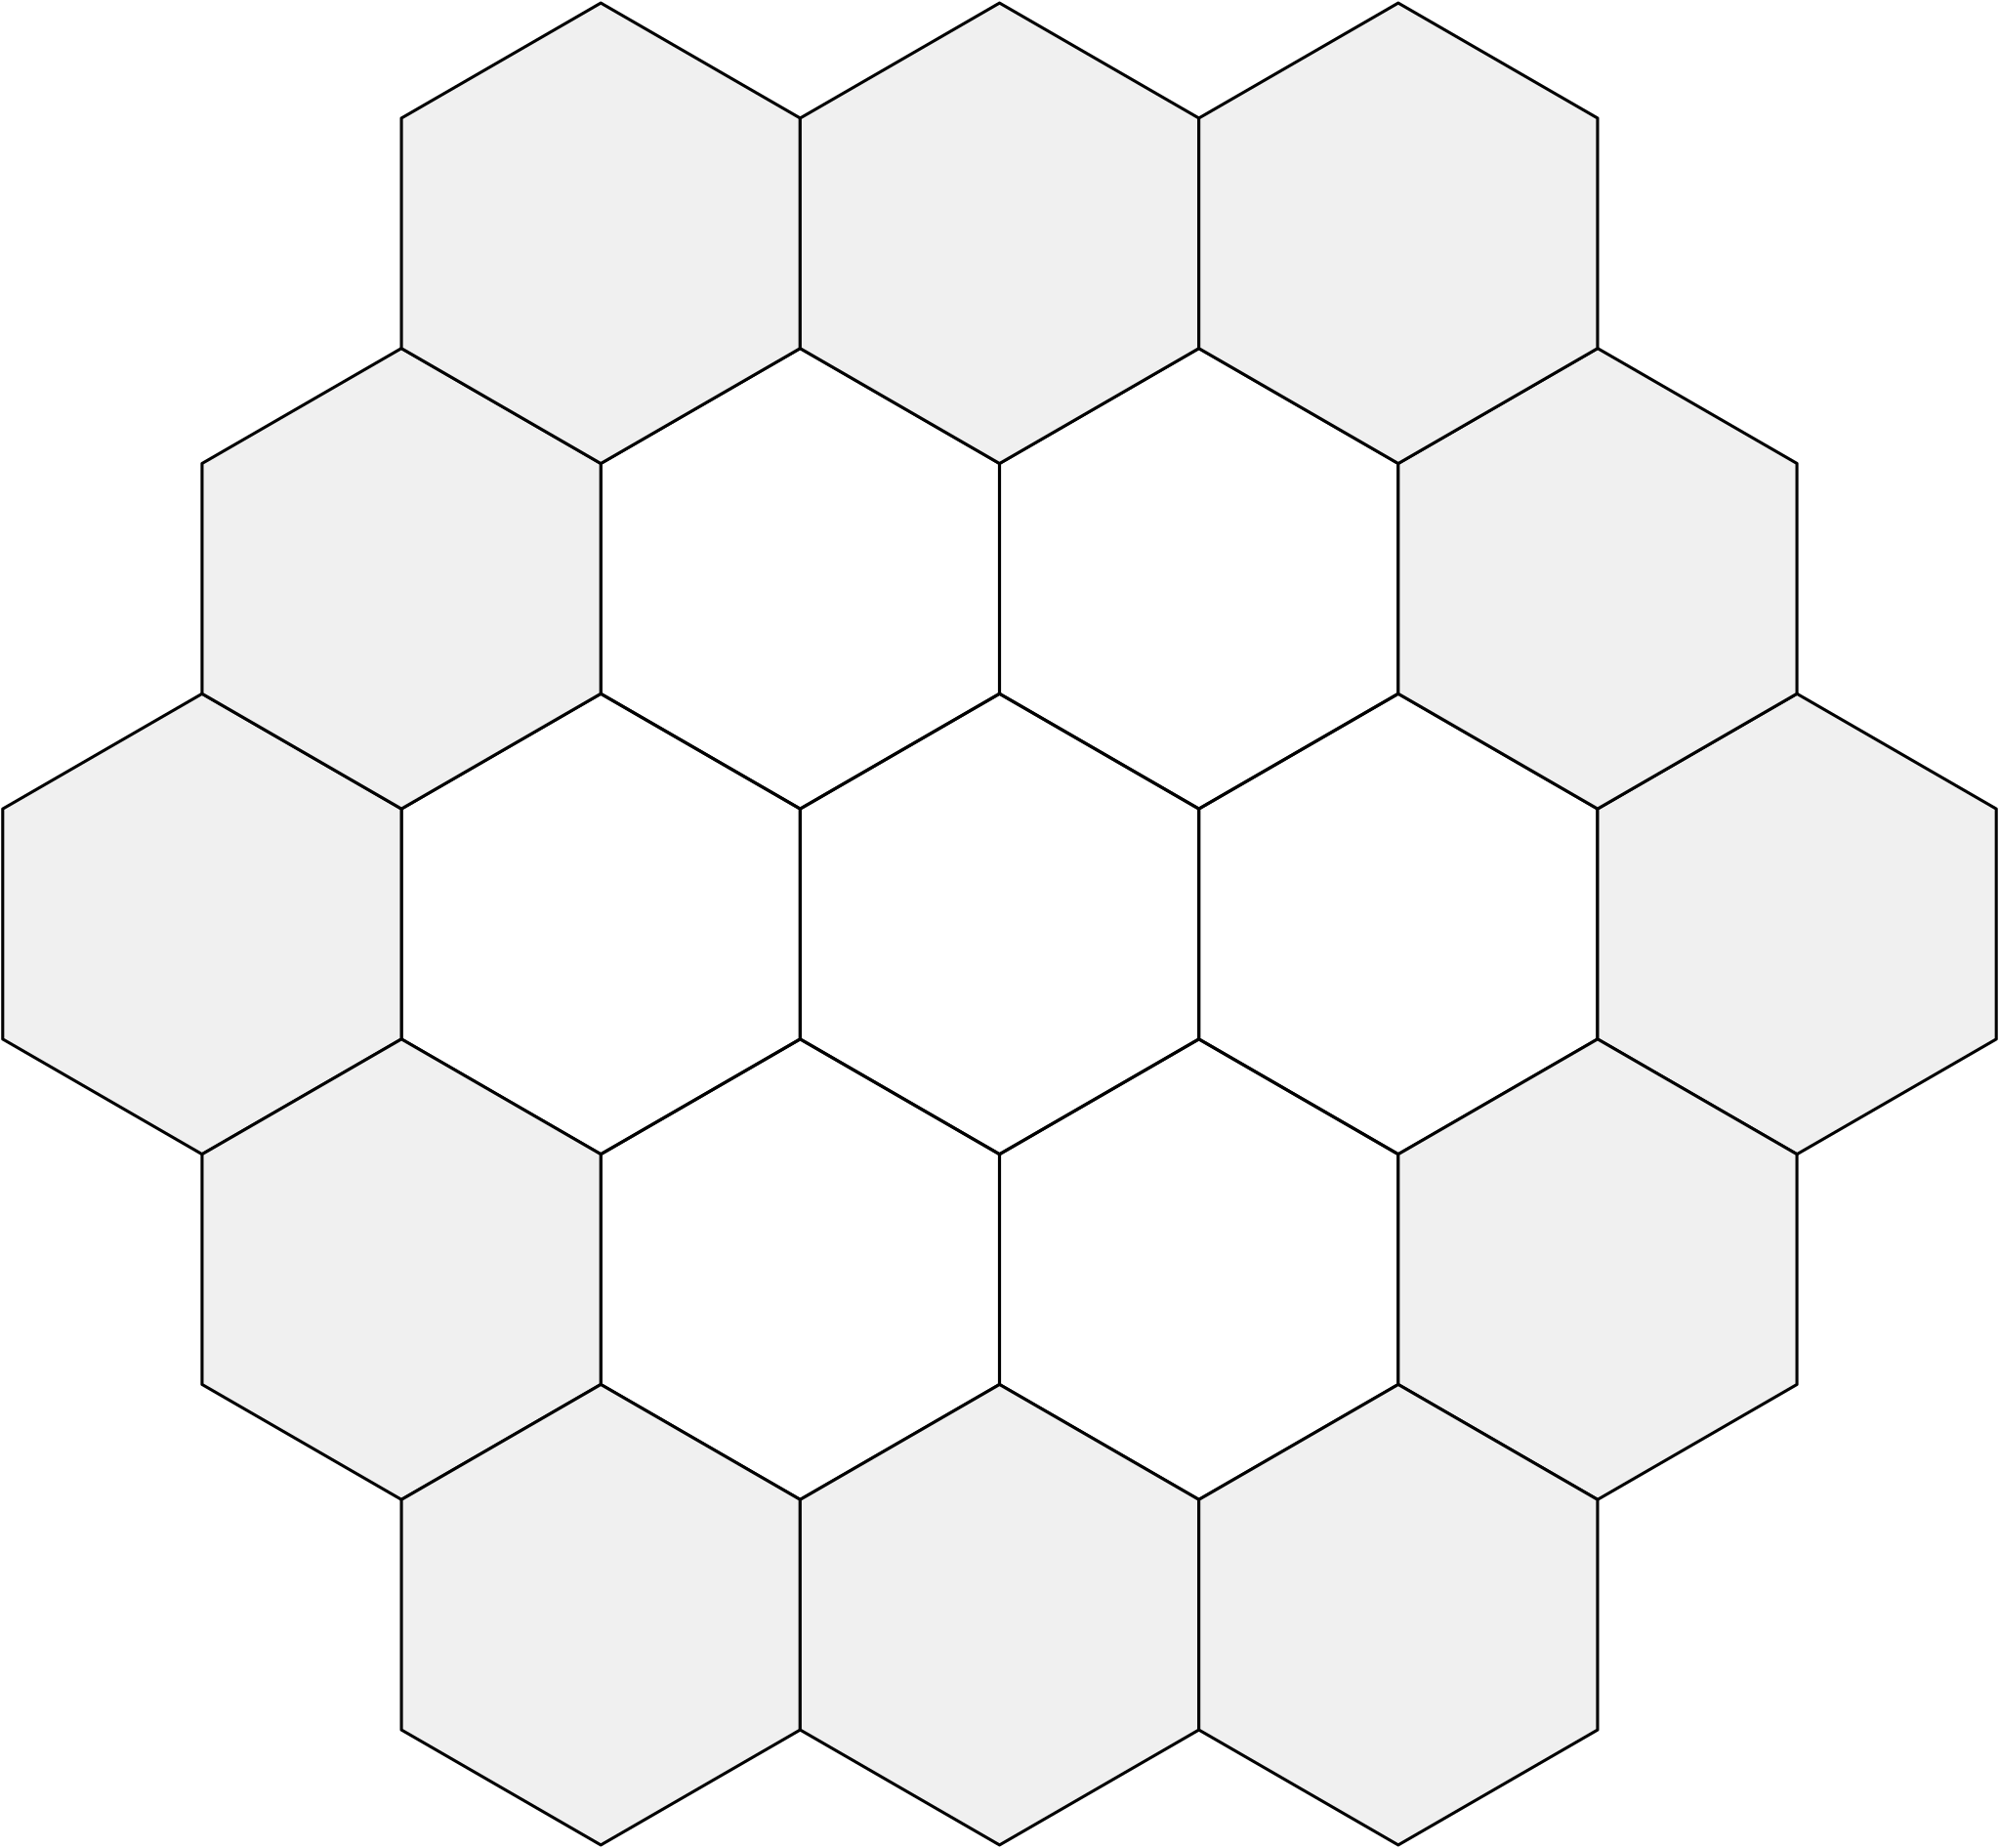
\includegraphics[width=0.75\columnwidth]{./figure/scenario}
\caption{The cells in the cluster (white) experience the OCI generated by the interfering cells (shaded).}
\label{fig:scenario}
\end{figure}

\begin{figure}[t]
\centering
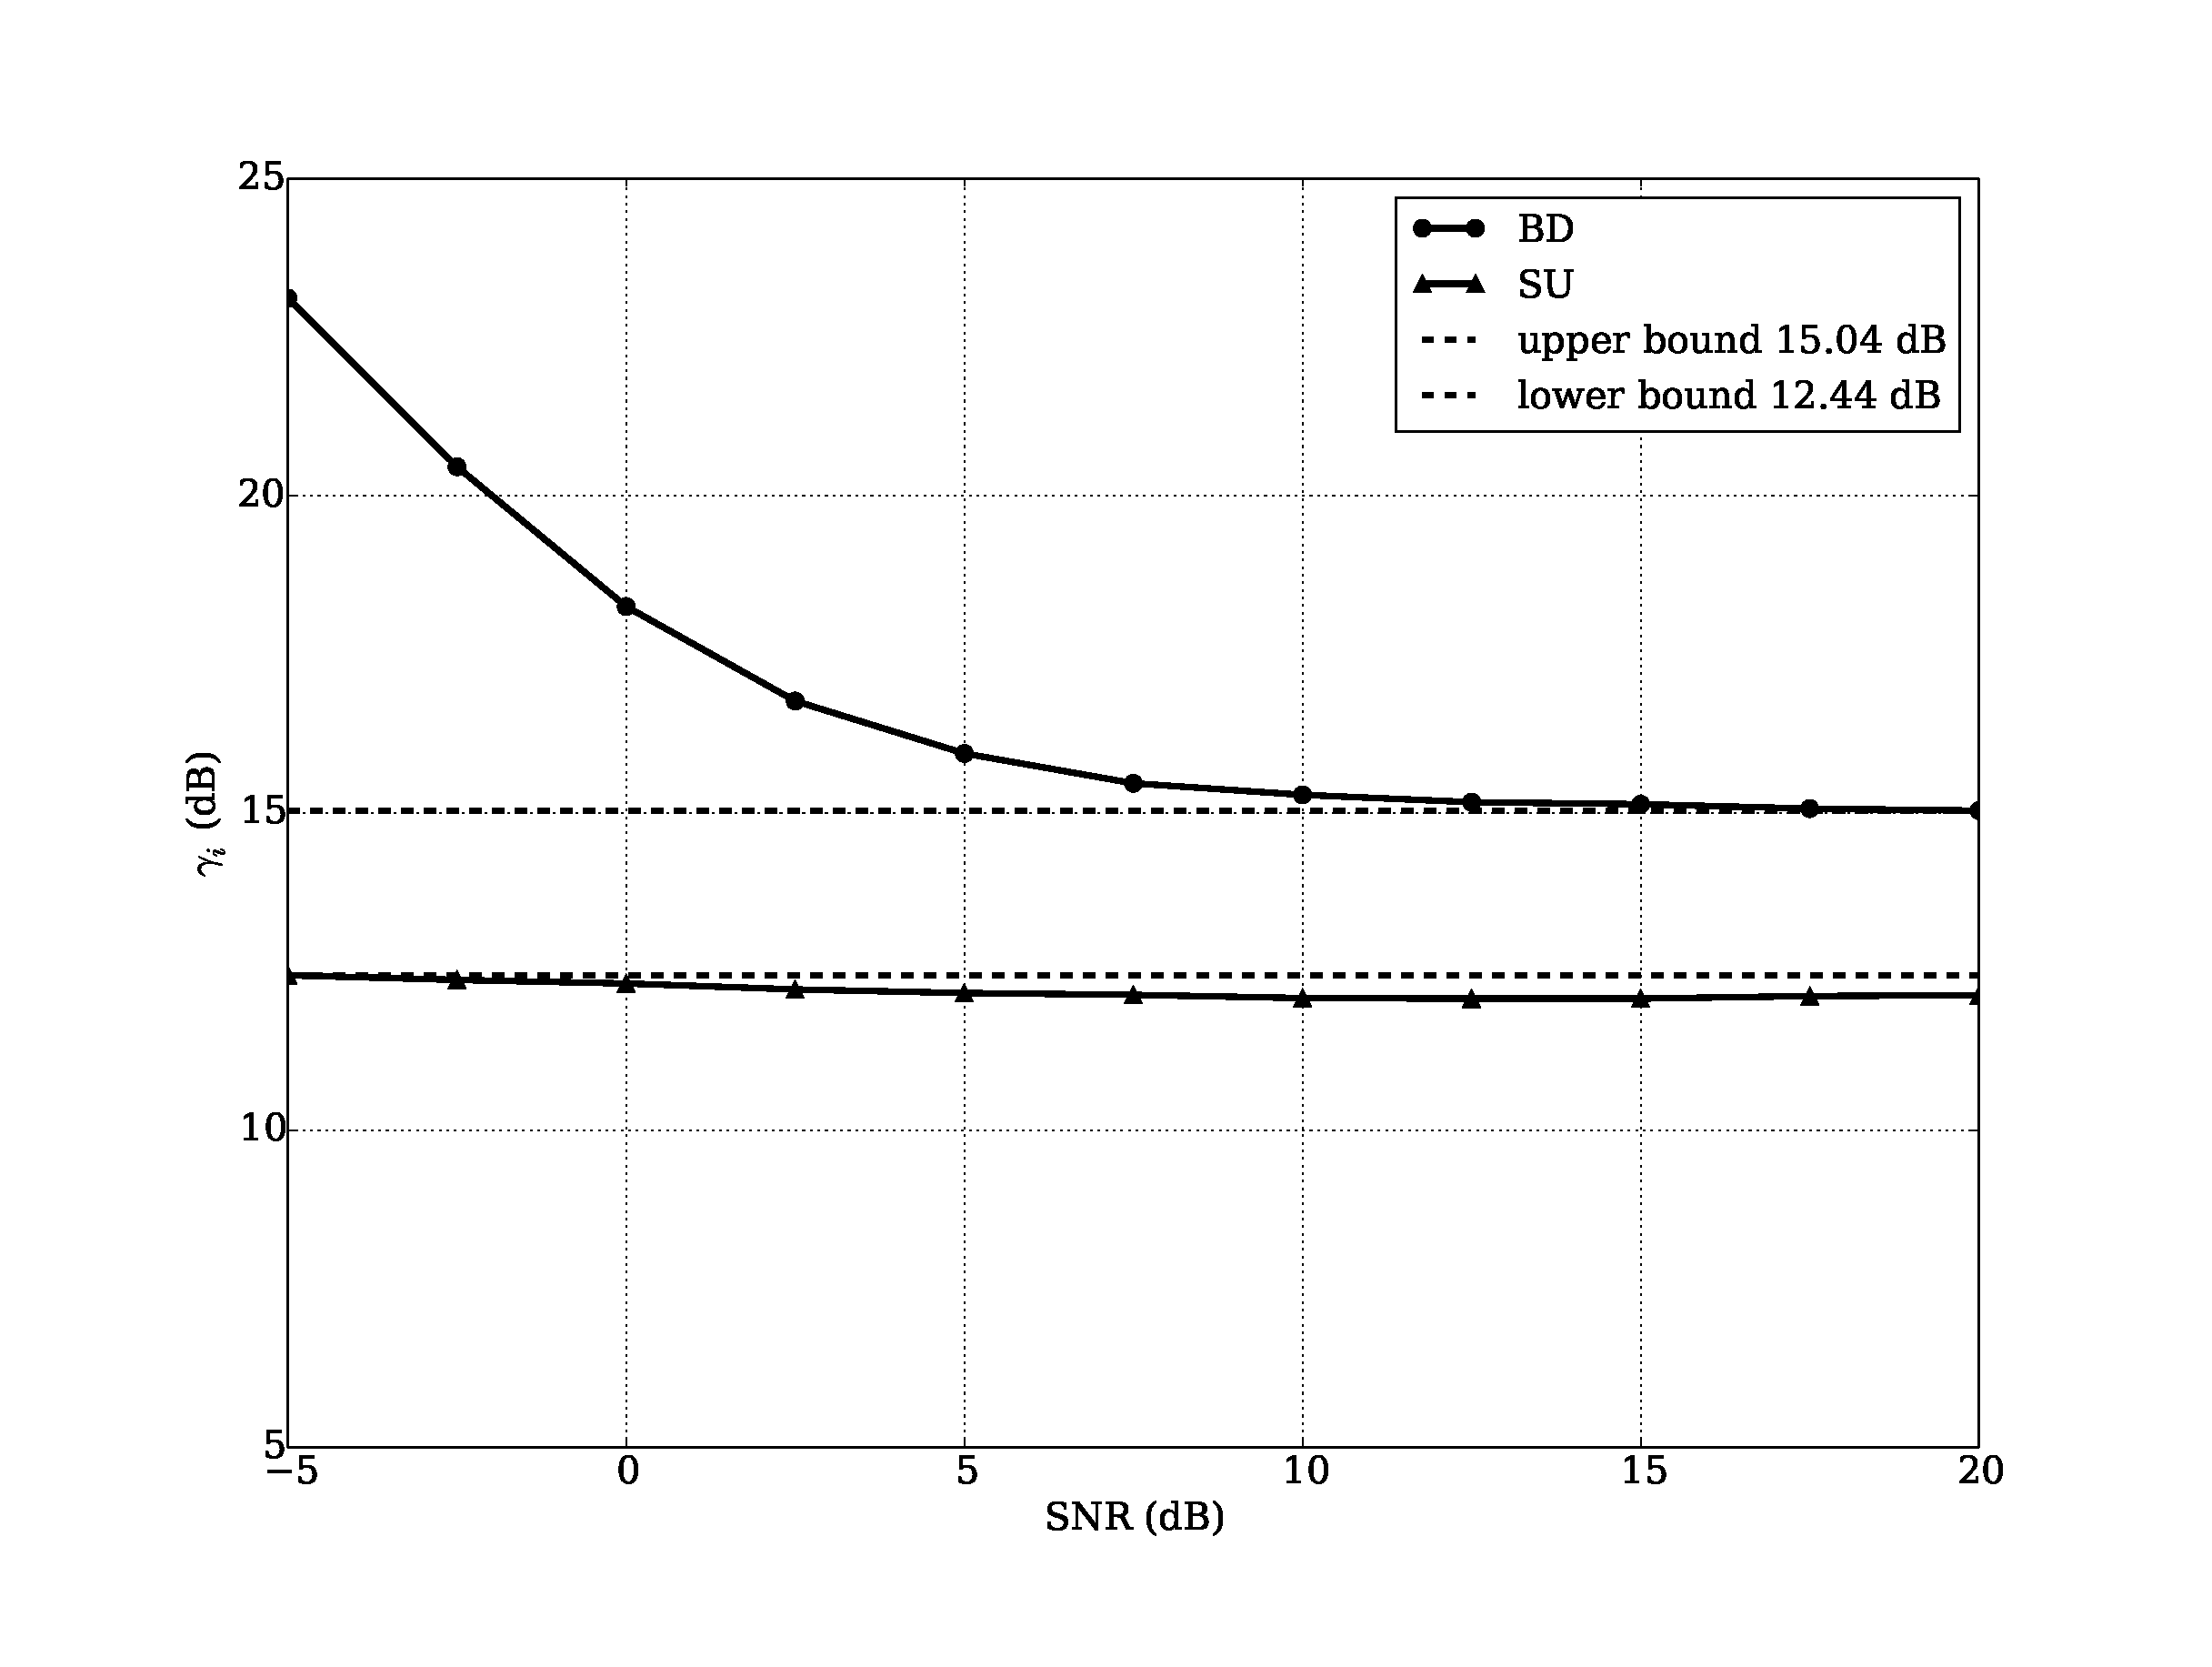
\includegraphics[width=1\columnwidth]{./figure/mean_metric_02x02}
\caption{Mean value of the metric for different SNR values, in the presence of OCI for a 7 cell cluster with 2x2 antennas configuration.}
\label{fig:threshold}
\end{figure}

The channel matrix includes both the path loss and the Rayleigh fast fading. Each of its coefficients is, therefore, a circularly symmetric complex gaussian random variable, with zero mean and variance given by the path loss, $\mathcal{CN}\left(0, \alpha(d)^{-1}\right)$, where $\alpha(d)$ represents the path loss in natural units, that depends on the distance from the BS to the user equipment, $d$.

The model used to calculate the path loss, in dB, is

\begin{equation}\label{eq:pathloss}
\text{PL}(d) = 10\log_{10} \alpha(d) = K + 10 \gamma \log_{10}\left(\frac{d}{d_0}\right)
\end{equation}

\noindent
with $K$ being the attenuation, in dB, at a reference distance of $d_0$, $\gamma$ is the path loss exponent. All the results in the paper correspond to a scenario with cell radius of $r_{cell} = 1380$\,m, path loss exponent equal to $3.8$, and $K=32$\,dB at a reference distance of $1$\,m.

The \emph{signal to noise ratio} (SNR) is calculated at the cell-edge using the maximum transmission power allowed per BS, $P_{max}=1$\,W, and the attenuation due to the path loss, as

\begin{equation}\label{eq:snr}
	\text{SNR\,(dB)} = 10\log_{10} P_{max} - \text{PL}(r_{cell})
\end{equation}

The rate is calculated for the following transmission options:

\begin{itemize}
\item All BS transmit using SU.
\item All BS transmit using BD.
\item The transmission strategy is chosen using the algorithm and scheduling proposed in this paper.
\item The same as the previous, but the scheduling is performed based on the rates obtained using BD, instead of the approximation in \eqref{eq:frobapprox}.
\end{itemize}

In all cases, the power assignment is done using the scaled-waterfilling described in \cite{zhang09}, in order to accomodate the per base power constraint.

\begin{figure}[t]
\centering
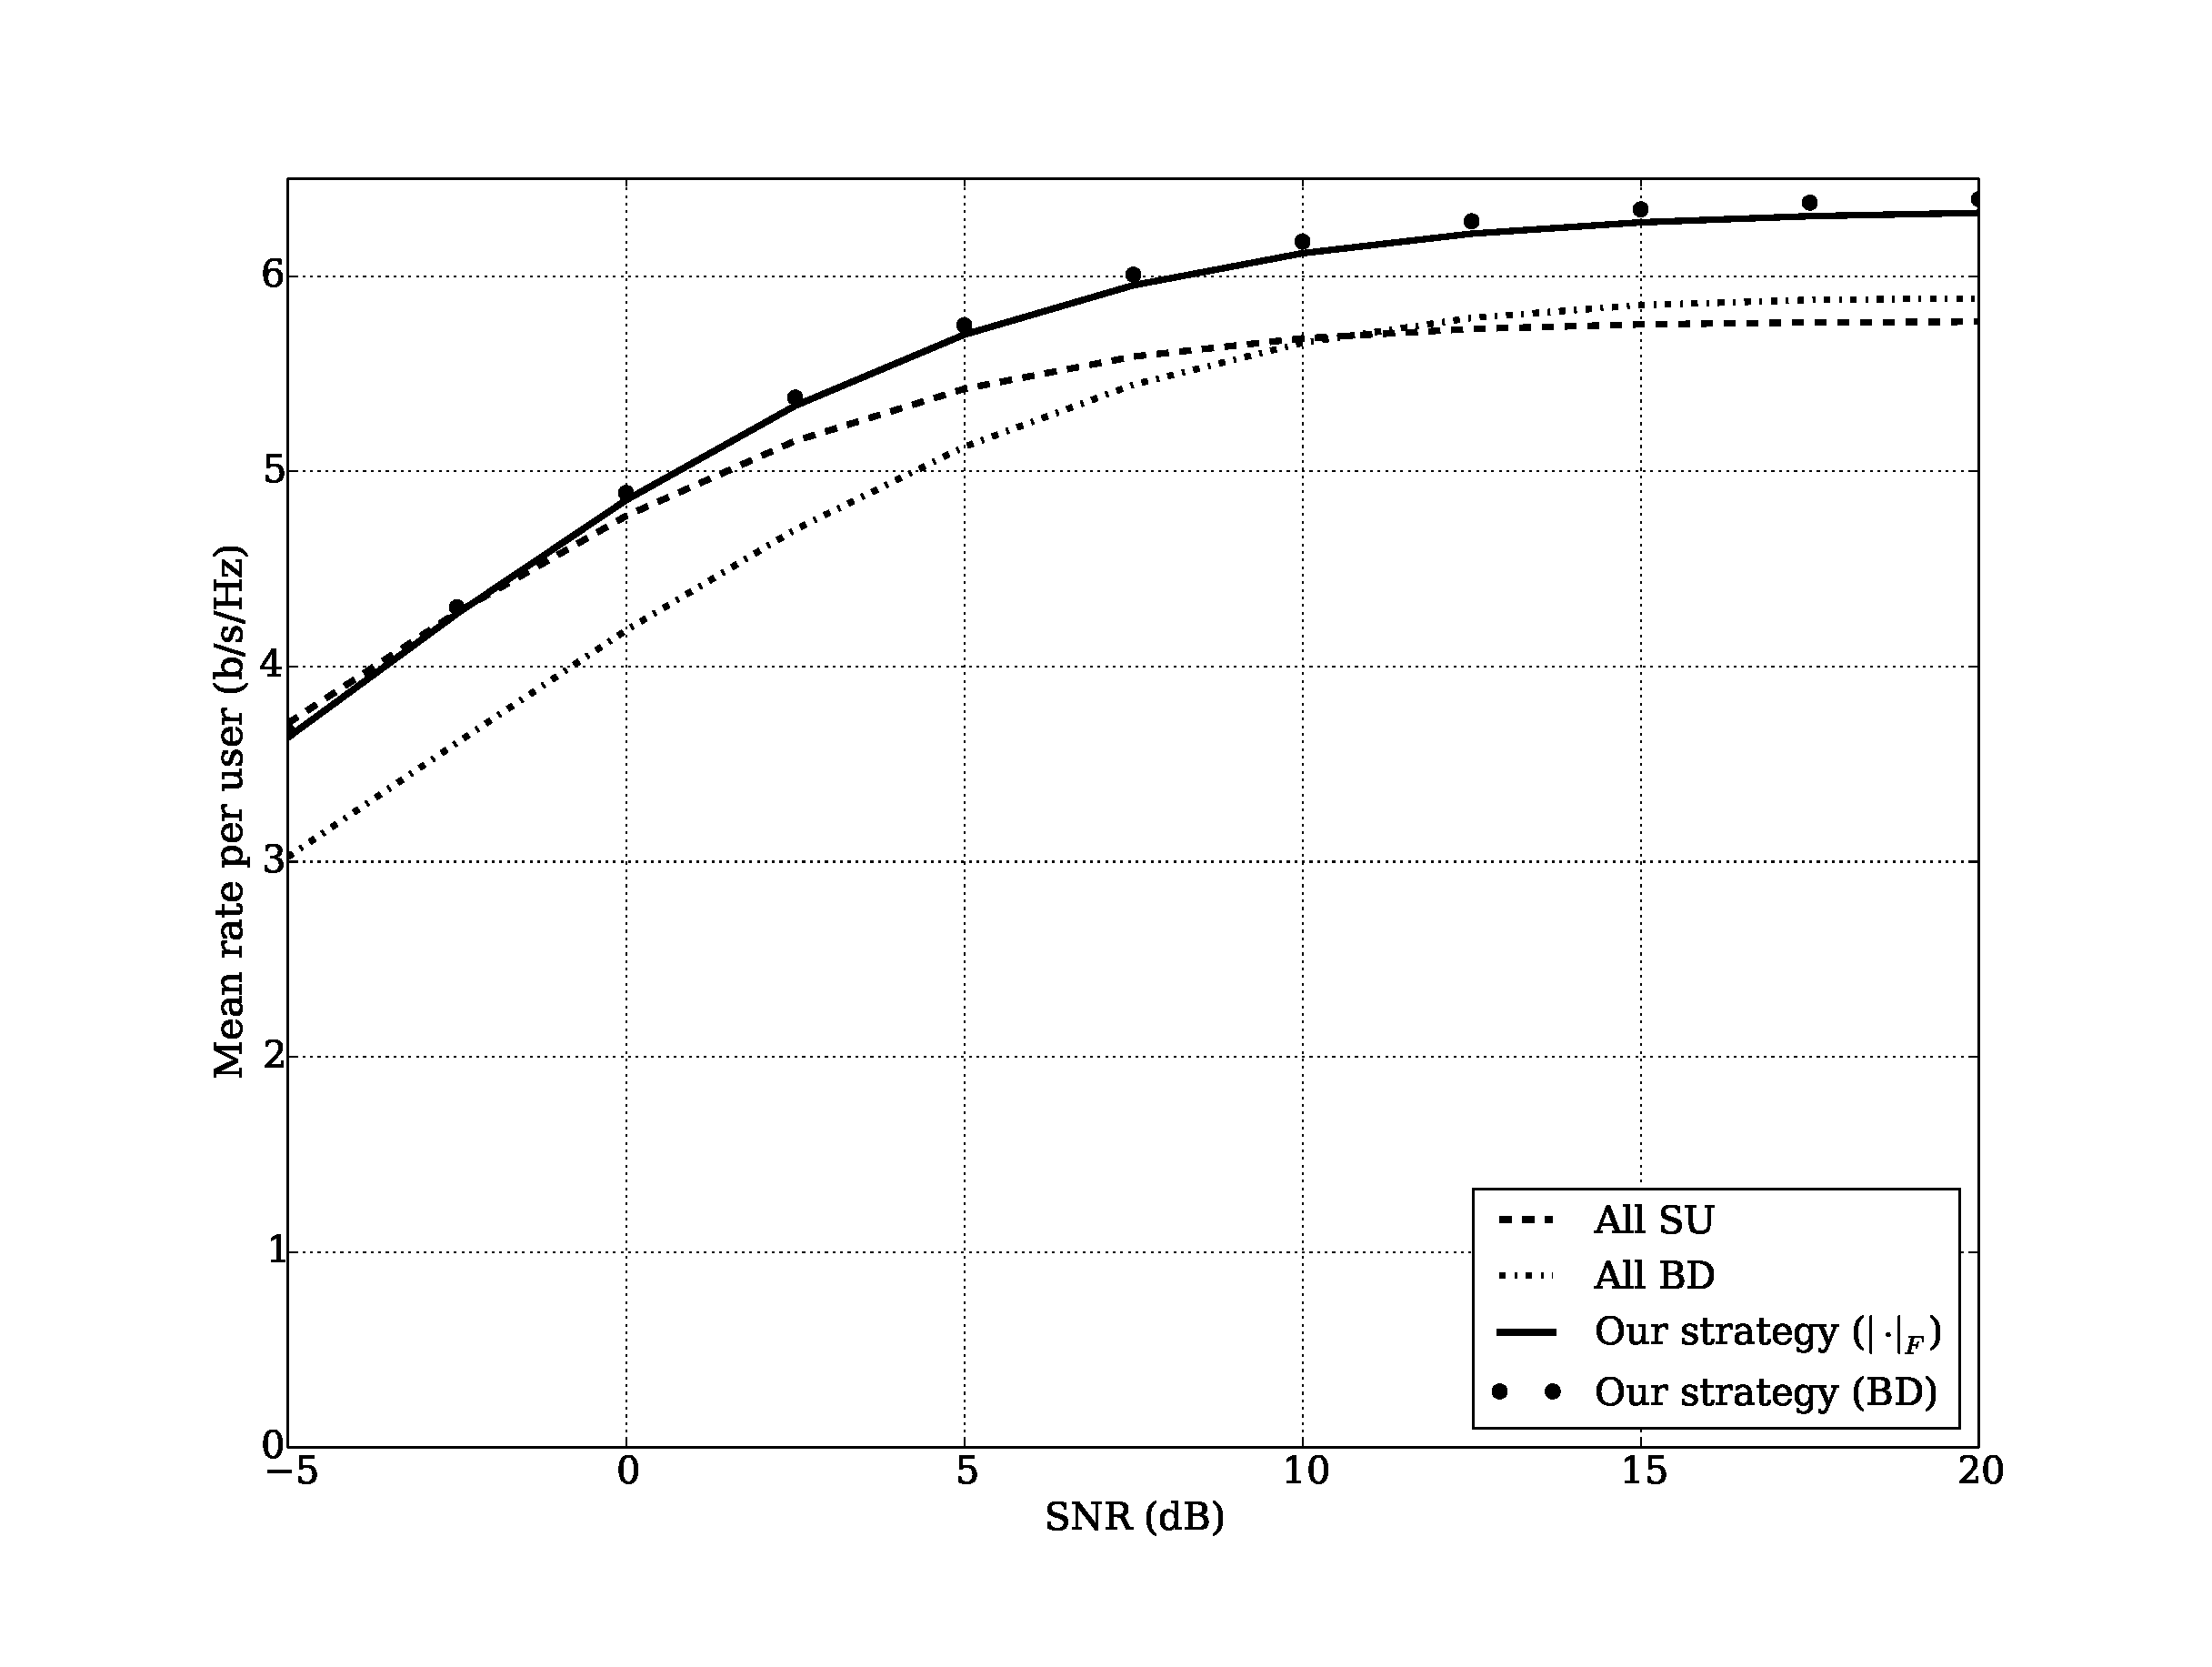
\includegraphics[width=1\columnwidth]{./figure/mean_rate_02x02_100user_bd}
\caption{Mean rate obtained for a 2x2 scenario in the presence of OCI, 100 users per cell.}
\label{fig:mean_rate_2x2}
\end{figure}

\begin{figure}[t]
\centering
\includegraphics[width=1\columnwidth]{./figure/mean_rate_03x03_100user_bd}
\caption{Mean rate obtained for a 3x3 scenario in the presence of OCI, 100 users per cell.}
\label{fig:mean_rate_3x3}
\end{figure}

\begin{figure}[t]
\centering
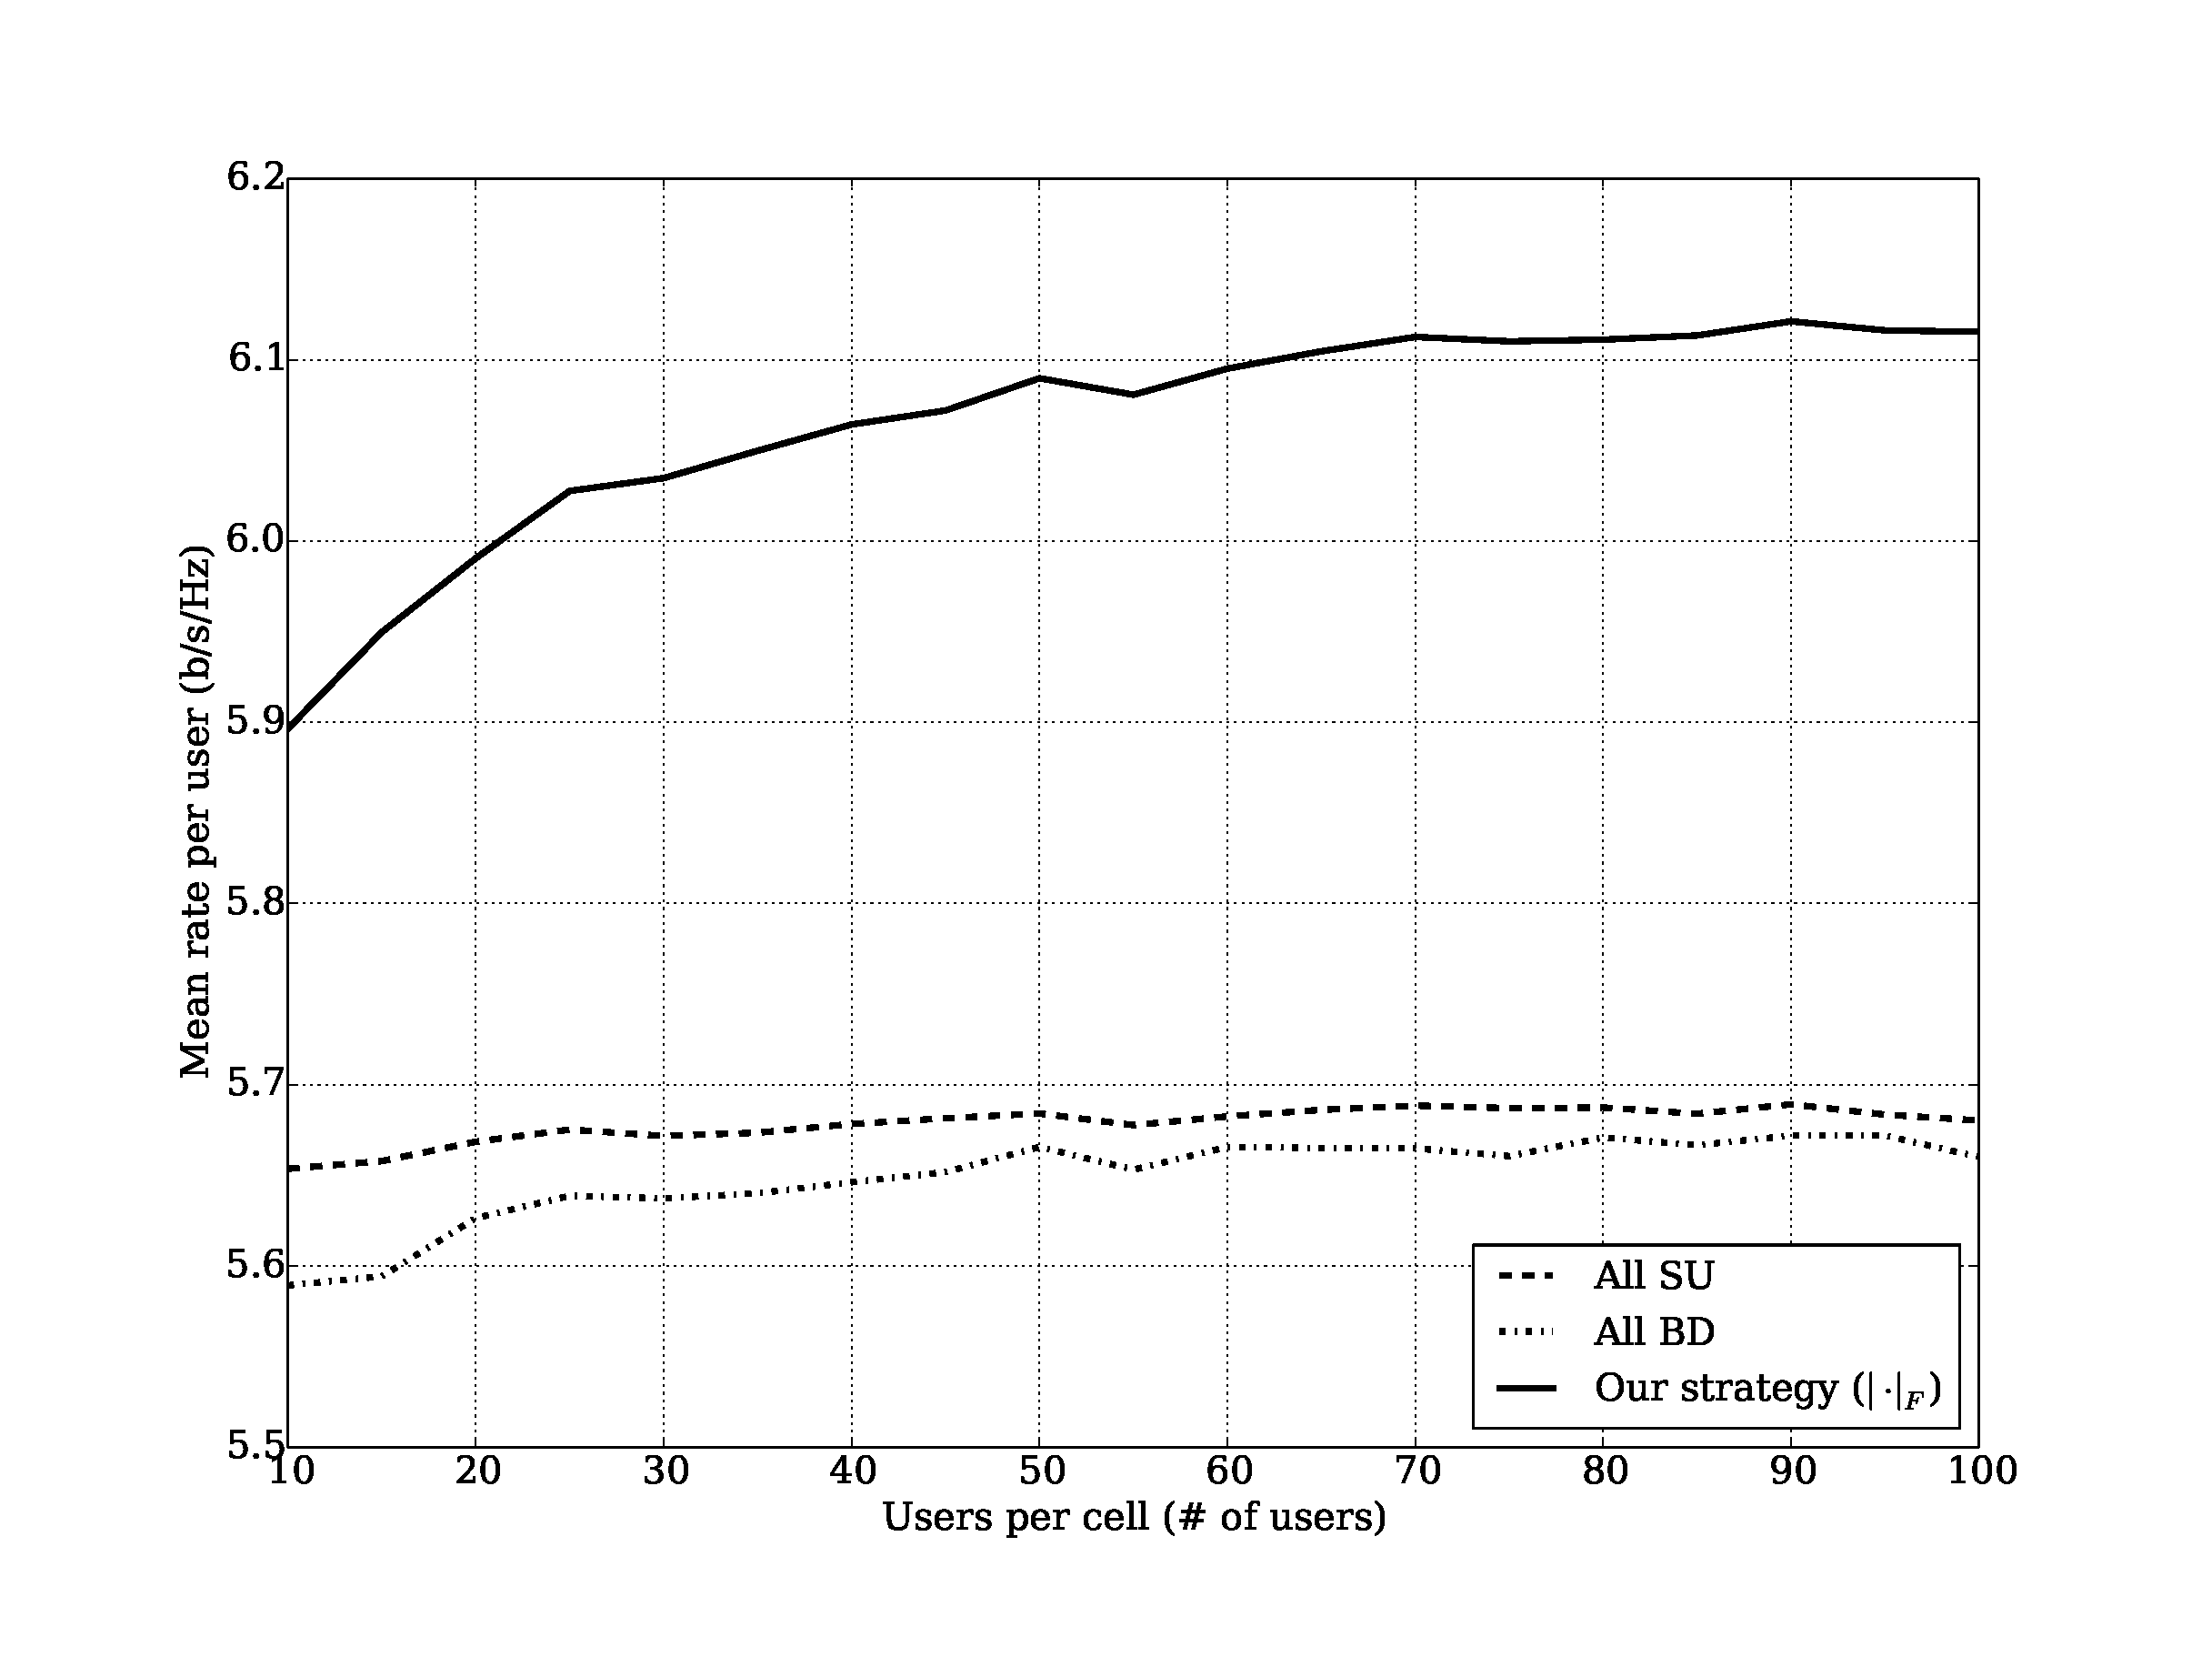
\includegraphics[width=1\columnwidth]{./figure/mean_rate_vs_users_02x02_s10}
\caption{Mean rate for a 2x2 scenario as a function of the number of users per cell, for an SNR of 10\,dB.}
\label{fig:mean_rate_vs_users}
\end{figure}

As mentioned in \refs{sec:transmission_strategy}, the threshold $\gamma_{th}$ is fixed and it is calculated via simulations. In these, a user is placed in each cell of the cluster, and the rate is calculated, both when all the BSs in the cluster coordinate to transmit using BD and when they transmit independently using SU, as well as the metric \eqref{eq:metric}. With this information \reff{fig:threshold} can be generated, where each of the solid-line curves in it represents the mean value of the metric \eqref{eq:metric}, in dB, for the users whose rate is better using BD and for those that get better results using SU, respectively. The threshold was calculated for a 2x2 MIMO case, but simulations were also performed with different number of antennas, keeping $t = r$, and the curves were similar, yielding the same threshold. 

The threshold $\gamma_{th}$ used in the simulations is determined as the mid value of the gap separating both curves in \reff{fig:threshold}. For the case at hand this value is $\gamma_{th} = 13.74$\,dB, but this value will depend on the scenario under study, and more simulations would be necessary in order to get this threshold for different number of cells and different network layouts.

\reff{fig:mean_rate_2x2} and \reff{fig:mean_rate_3x3} show the mean rate that can be achieved, per user, for the transmission options considered. It can be seen how accurate is the approximation \eqref{eq:frobapprox}, while being notably simpler and much less computationally expensive.

\reff{fig:mean_rate_vs_users} shows the mean rate of the three scenarios for a fixed SNR of $10$\,dB, for a variable number of users per cell. The proposed scheme is able to surpass the performance of the SU strategy, and the improvement increases with the number of users.

\reff{fig:cdf_snr10} and \reff{fig:worst_rate} show a more severe problem of BD in presence of OCI, which is the fairness of the solution. \reff{fig:cdf_snr10} represents the \emph{cummulative distribution function} (CDF) of the rates obtained with each of the transmission strategies for a fixed value of the SNR. It can be seen how the rates obtained using the proposed strategy are higher, especially for the users with the lowest rates, which indicates an improvement in the fairness of the system. \reff{fig:worst_rate} shows the average rate for the 5\% worst users, showing a clear improvement using the strategy proposed in this paper with respect to using only BD, and matching the average rate obtained with the SU strategy.

\begin{figure}[t]
\centering
\includegraphics[width=1\columnwidth]{./figure/cdf_02x02_s20_100user_bd} \caption{CDF of the rates obtained in a 2x2 scenario, with an SNR of $10$\,dB.}
\label{fig:cdf_snr10}
\end{figure}

\begin{figure}[t]
\centering
\includegraphics[width=1\columnwidth]{./figure/mean_rate_005_worst_02x02_100user_bd} \caption{Mean rate of the 5\% worst users, in a 2x2 scenario in the presence of OCI, 100 users per cell.}
\label{fig:worst_rate}
\end{figure}

%%%%%%%
\section{Conclusions}\label{sec:conclusions}
In this paper, a simple yet effective algorithm has been proposed in order to overcome the impairments introduced by the OCI in a clustered cellular network. The negative effect of the OCI in coordination techniques like BD is eliminated, and the fairness of the system is also improved. In particular, the mean rate per user is better than with SU, especially for a high number of users per cell. The improvement with respect to BD in the case of the users with the lowest achievable rate is notable, getting closer to SU.

An important advantage of the proposed scheme is its adaptive nature, as the users are responsible for choosing the technique used for the transmission, and the network will carry out the scheduling, so that a user will be able to change its transmission preferences when its conditions change.

It has been shown how the use of a simple fixed threshold can yield a better performance, at a very low computational cost. An interesting topic would be to analyze the relation of the threshold value with the network topology, so that the estimation through simulations can be avoided.

The proposed algorithm improves the fairness of the system, especially for the users that experience the lowest rates. A possible extension is to use a proportional fair approach for the scheduling, instead of the simple round robin, so that more fairness can be induced in the system.

%%% BIBLIOGRAPHY %%%%%%%%%
\bibliographystyle{ieeetr}
\bibliography{ew2014_jjgarcia}

\end{document}
